\documentclass{standalone}
\usepackage{tikz}
\usepackage{amssymb}

\begin{document}
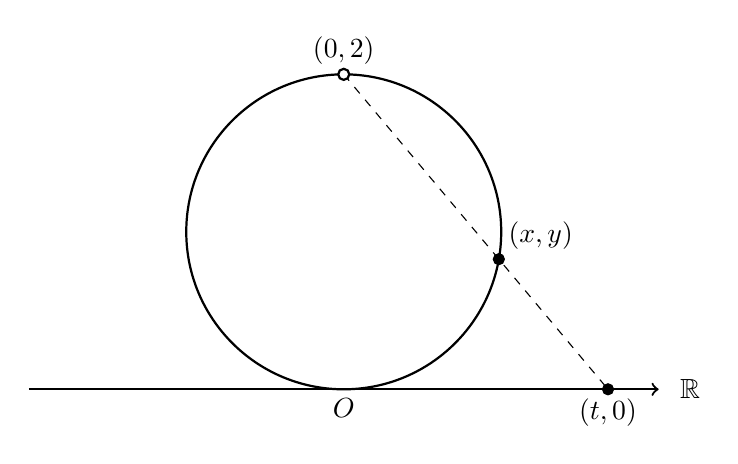
\begin{tikzpicture}[scale=2]

    % Окружность с центром в (0, 1) и радиусом 1
    \draw[thick] (0, 1) circle (1);

    % Прямая (ось Ox)
    \draw[thick, ->] (-2, 0) -- (2, 0) node[right] {$$};

    % Полюс проекции (выколотая точка)
    \node[above] at (0, 2) {$(0, 2)$};

    % Точка на окружности
    \def\theta{100} % Угол в градусах
    \pgfmathsetmacro\x{sin(\theta)}
    \pgfmathsetmacro\y{1 + cos(\theta)}
    \filldraw (\x, \y) circle (1pt) node[above right] {$(x, y)$};

    % Линия проекции (исправленная формула)
    \pgfmathsetmacro\t{(2*\x)/(2 - \y)}
    \draw[dashed] (0, 2) -- (\x, \y) -- (\t, 0);

    \fill[white] (0, 2) circle (1pt); % Белая заливка
    \draw[thick] (0, 2) circle (1pt); % Пустая окружность

    % Точка на прямой
    \filldraw (\t, 0) circle (1pt) node[below] {$(t, 0)$};

    % Подписи
    %\node at (0, 1.2) {$S^1$};
    \node[below] at (0, 0) {$O$};
    \node at (2.2, 0) {$\mathbb{R}$};
\end{tikzpicture}
\end{document}